\section{Vizuelizacija}
\label{sec:Vizuelizacija}

U ovom odeljku \'c{}emo poku\v{s}ati da \v{c}itaocu damo vizuelni prikaz raznovrsnosti skupa podataka, uz osvrt na neke zanimljive zaklju\v{c}ke. Neki od atributa koji su vizuelizovani u ovom odeljku nisu u potpunosti prisutni u skupu, tako da je analiza takvih atributa radjena samo nad slogovima gde nema nedostaju\'c{}ih vrednosti za te atribute.

Vizuelizacija originalnog skupa podataka je prikazana na slici \ref{fig:before}. Nedostaju\'c{}e vrednosti su prikazane belom bojom, dok su plavom bojom predstavljene postoju\'c{}e vrednosti atributa.
\begin{figure}[H]
    \centering
    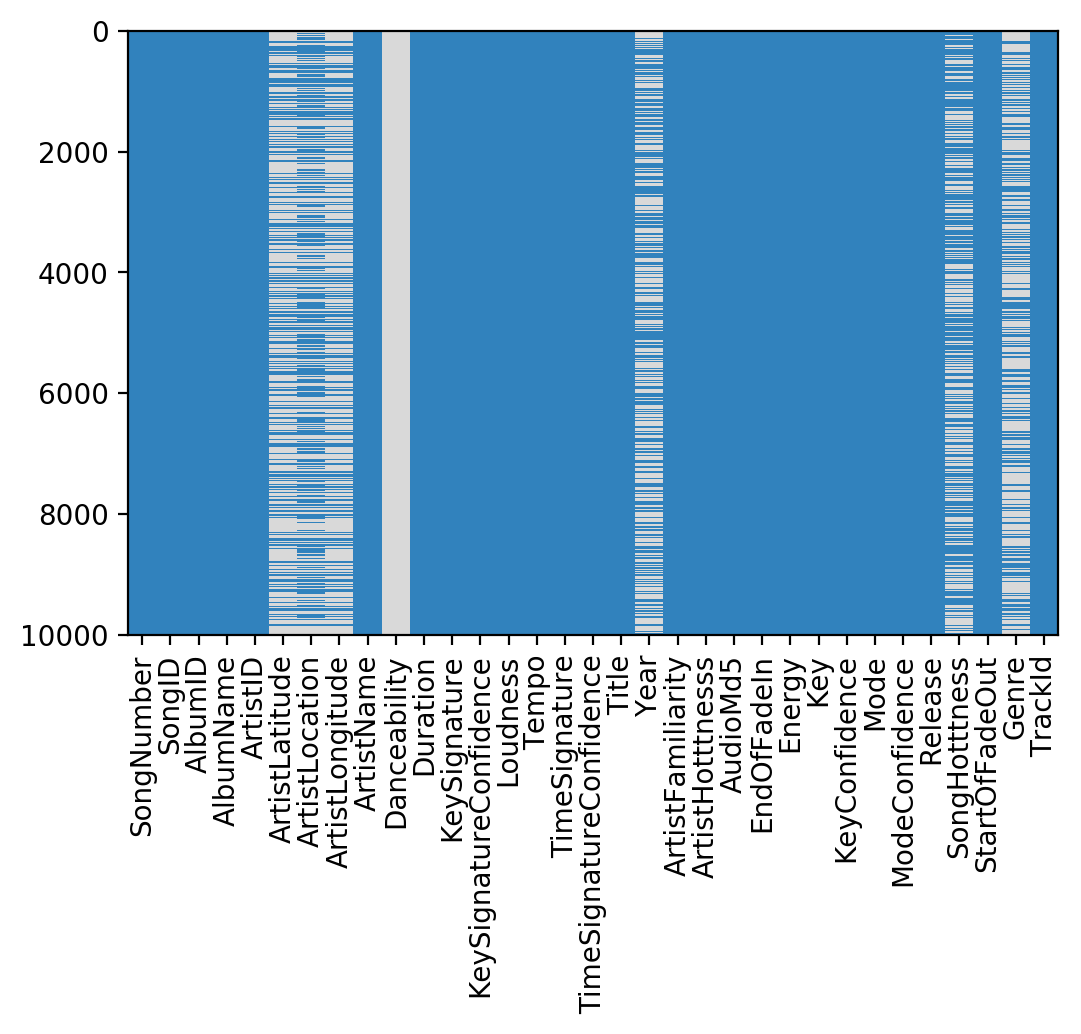
\includegraphics[scale=0.6]{resources/before_processing.png}
    \label{fig:before}
    \caption{Originalni skup podataka}
\end{figure}

 Sa prikaza skupa podataka se vidi da atribut koji opisuje plesnu mo\'c{} pesme \emph{eng. dancability}, ni u jednom slu\v{c}aju nema postavljenu vrednost, te da je on neupotrebljiv. Takodje, godina, lokacija autora, geografska \v{s}irina, geografska du\v{z}ina i \v{z}anr su atributi koji u velikom broju slu\v{c}ajeva nemaju vrednost. Medjutim, zbog njihove va\v{z}nosti, mi \'c{}emo svoje istra\v{z}ivanje vr\v{s}iti nad onim slogovima za koje su ove vrednosti poznate. Nakon izdvajanja relevantnih atributa za na\v{s}e istra\v{z}ivanje, pripremljen skup podataka je prikazan na slici \ref{fig:after}.
 
\begin{figure}[H]
    \centering
    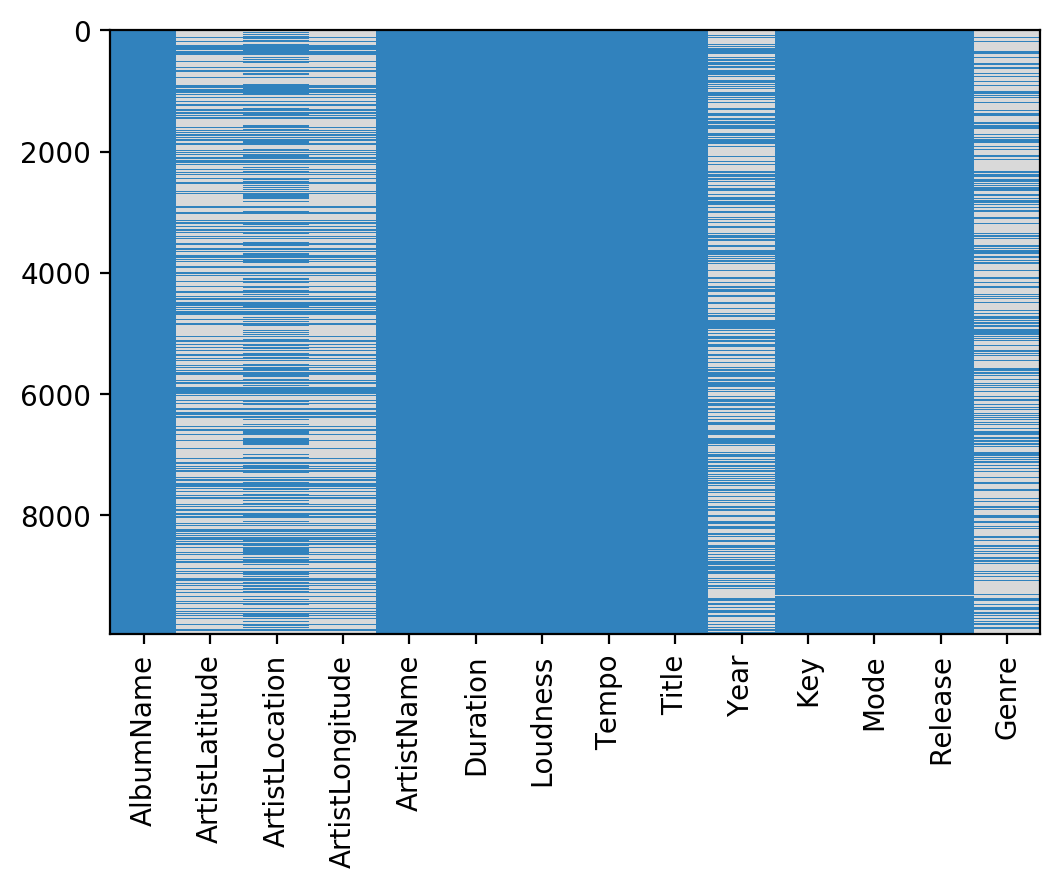
\includegraphics[scale=0.6]{resources/after_processing.png}
    \label{fig:after}
    \caption{Izdvojeni atributi kori\v{s}\'c{}eni u istra\v{z}ivanju}
\end{figure}

// TODO outliers

Geografska rasprostranjenost autora \v{c}ije su se pesme na\v{s}le u skupu podataka se mo\v{z}e videti na slici \ref{fig:Geolokacija}. Razli\v{c}ite boje predstavljaju vizuelizaciju godine izdavanja pesme - gradijentni prelaz od plave (1950) do crvene (2010).

\begin{figure}[H]
    \centering
    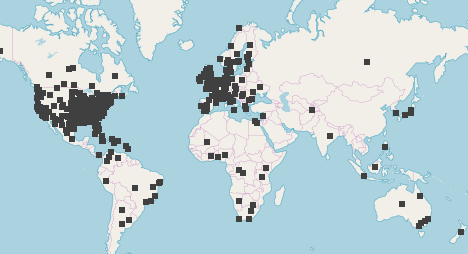
\includegraphics[scale=0.45]{resources/Geolokacija.png}
    \label{fig:Geolokacija}
    \caption{Geografska rasprostranjenost autora}
\end{figure}

Spisak najzastupljenijih zanrova u skupu se mo\v{z}e videti na slici \ref{fig:ZastupljenostZanrova}. \v{Z}anr je atribut sa velikom stopom nedostaju\'c{}ih vrednosti, uz dodatni problem re\v{c}enica prisutnih u nizu (podse\'c{}amo na problem naveden prilikom preprocesiranja, poglavlje \ref{sec:Preprocesiranje}), tako da je analiza vr\v{s}ena nad veoma ograni\v{c}enim skupom od oko tri hiljade slogova. Smatramo, da su ovi rezultati u velikoj meri sli\v{c}ni rezultatima koji bi se dobili da je potpuni skup analiziran - ukoliko ne bi bilo nedostaju\'c{}ih vrednosti za atribut \v{z}anr.

Grafik zavisnosti godine i trajanja pesme se mo\v{z}e videti na slici \ref{fig:YearDuration}. Jedan zanimljiv zaklju\v{c}ak koji se name\'c{}e, je da se prose\v{c}no trajanje pesama pove\'c{}ava kroz vreme, sa razlikom od oko 20 sekundi u odnosu na 50-te godine pro\v{s}log veka. Detaljniji prikaz promene proseka trajanja se mo\v{z}e videti na slici \ref{fig:YearDurationAvg}. Takodje, jasno je da se i raznovrsnost pesama mnogo ve\'c{}a danas - prisutne su i veoma kratke ali i veoma duga\v{c}ke pesme.

\begin{figure}[H]
    \centering
    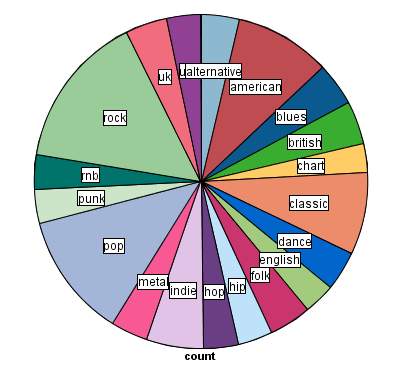
\includegraphics[scale=0.5]{resources/ZastupljenostZanrova.png}
    \caption{Zastupljenost \v{z}anrova}
    \label{fig:ZastupljenostZanrova}
\end{figure}

\begin{figure}[H]
    \centering
    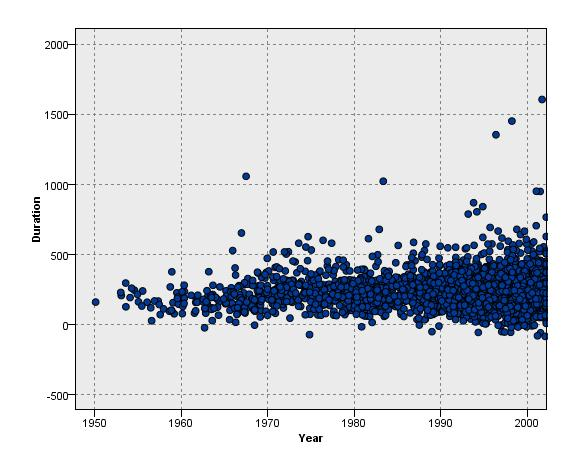
\includegraphics[scale=0.6]{resources/year-duration.jpg}
    \caption{Odnos godine izdavanja i du\v{z}ine pesme}
    \label{fig:YearDuration}
\end{figure}

\begin{figure}[H]
    \centering
    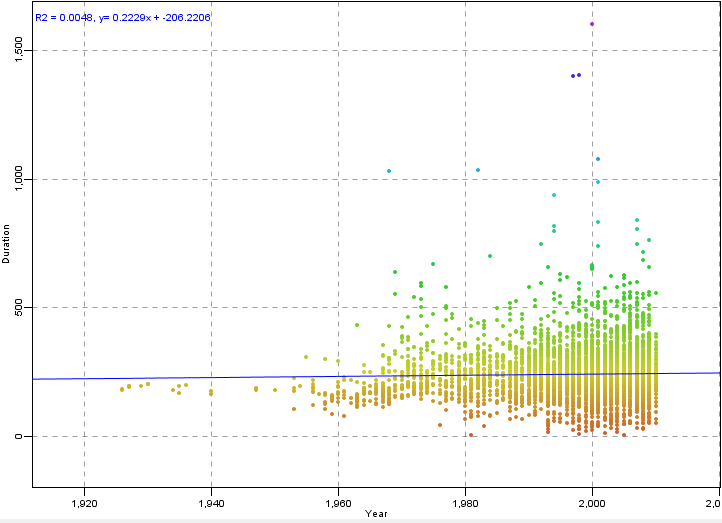
\includegraphics[scale=0.6]{resources/year-duration.PNG}
    \caption{Promena proseka du\v{z}ine pesama kroz vreme}
    \label{fig:YearDurationAvg}
\end{figure}
